\documentclass[journal]{IEEEtran}

% ── Packages ──────────────────────────────────────────────
\usepackage[T1]{fontenc}
\usepackage{amsmath,amssymb,amsfonts,amsthm}
\usepackage{algorithmic}
\usepackage{algorithm}
\usepackage{graphicx}
\usepackage{textcomp}
\usepackage{booktabs}
\usepackage{multirow}
\usepackage{cite}
\usepackage{url}
\usepackage{color}
\usepackage{bm}
\usepackage{siunitx}
\usepackage{tikz}
\usetikzlibrary{arrows.meta, positioning, shapes.geometric, fit, calc}

% ── Math shortcuts ────────────────────────────────────────
\newtheorem{theorem}{Theorem}
\newcommand{\vx}{\mathbf{x}}
\newcommand{\vz}{\mathbf{z}}
\newcommand{\vP}{\mathbf{P}}
\newcommand{\vQ}{\mathbf{Q}}
\newcommand{\vR}{\mathbf{R}}
\newcommand{\vH}{\mathbf{H}}
\newcommand{\vK}{\mathbf{K}}
\newcommand{\vI}{\mathbf{I}}
\newcommand{\vF}{\mathbf{F}}
\newcommand{\vS}{\mathbf{S}}
\newcommand{\tr}{\operatorname{tr}}

\begin{document}

% ══════════════════════════════════════════════════════════
%  TITLE
% ══════════════════════════════════════════════════════════
\title{BLOCS: Building Localization with Observer-Based\\Control Strategy for UAVs}

\author{Muhammed~Emin~Kaya%
\thanks{M.~E.~Kaya is with the Department of Control and Automation Engineering, Yildiz Technical University, Istanbul, Turkey (e-mail: \texttt{eminkaya@yildiz.edu.tr}).}}

\markboth{IEEE Robotics and Automation Letters, 2026}{}

\maketitle

% ══════════════════════════════════════════════════════════
%  ABSTRACT
% ══════════════════════════════════════════════════════════
\begin{abstract}
Accurate localization of buildings from unmanned aerial vehicles (UAVs) using monocular cameras is fundamental to urban mapping, search-and-rescue, and infrastructure inspection.
Existing approaches rely on direct odometry-based inverse projection at a fixed flight altitude, which suffers from cumulative drift and an inherent accuracy--coverage tradeoff.
We present \textsc{BLOCS}, a framework that combines an Extended Kalman Filter (EKF) for static building position estimation with an uncertainty-driven altitude controller that adapts the UAV's height in real time based on the filter covariance.
We derive the measurement Jacobian for a pinhole camera model, prove observability conditions linking trajectory geometry to estimation quality, and show that circular trajectories yield an~$8\times$ improvement in condition number over straight-line approaches.
Monte~Carlo experiments over ten random seeds demonstrate sub-meter localization accuracy (\SI{0.16}{m} RMSE) under circular flight and graceful degradation with increasing pixel noise (\SI{0.11}{m} at $\sigma{=}1\,$px to \SI{0.44}{m} at $\sigma{=}10\,$px).
The adaptive altitude controller successfully balances exploitation (descending for accuracy) and exploration (ascending for coverage).
\end{abstract}

\begin{IEEEkeywords}
UAV, building localization, Extended Kalman Filter, active perception, observability, altitude control
\end{IEEEkeywords}

% ══════════════════════════════════════════════════════════
%  I. INTRODUCTION
% ══════════════════════════════════════════════════════════
\section{Introduction}
\IEEEPARstart{U}{nmanned} aerial vehicles equipped with monocular cameras are increasingly deployed for urban mapping, disaster assessment, and infrastructure monitoring~\cite{nex2014uav}.
A core capability these missions require is accurate three-dimensional localization of buildings observed from the air.

The prevailing approach, exemplified by the QUASAR system, detects buildings with a deep-learning object detector (YOLOv8~\cite{jocher2023yolov8}) and projects the bounding box center onto the ground plane using the UAV's onboard odometry.
While simple, this pipeline has two critical shortcomings:
\begin{enumerate}
    \item \textbf{Odometry drift.}  Position errors accumulate over time, directly corrupting the inverse projection.
    \item \textbf{Fixed altitude.}  Flying at a constant height ignores the fundamental tradeoff between measurement accuracy (which improves at lower altitude) and spatial coverage (which improves at higher altitude).
\end{enumerate}

This paper addresses both limitations.  We propose \textsc{BLOCS} (Building Localization with Observer-based Control Strategy), which makes three contributions:

\begin{enumerate}
    \item An \textbf{EKF formulation} for estimating static building positions from sequential monocular detections, using the Joseph-form covariance update for numerical stability and Mahalanobis gating for outlier rejection.
    \item A formal \textbf{observability analysis} that links UAV trajectory geometry to estimation quality through the observability Gramian, identifying degenerate motions analytically.
    \item An \textbf{adaptive altitude controller} that maps the EKF covariance trace to a desired altitude via an exponential control law with rate limiting, balancing exploitation and exploration in real time.
\end{enumerate}

% ── System Architecture Figure (full width) ───────────────
\begin{figure*}[t]
\centering
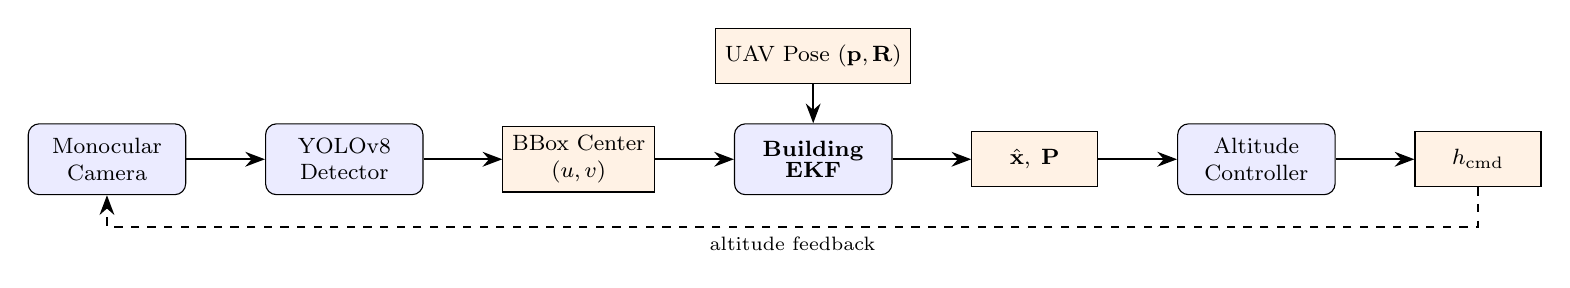
\begin{tikzpicture}[
    node distance=0.8cm and 1.0cm,
    block/.style={rectangle, draw, rounded corners, fill=blue!8, minimum height=0.9cm, minimum width=2.0cm, align=center, font=\footnotesize},
    data/.style={rectangle, draw, fill=orange!10, minimum height=0.7cm, minimum width=1.6cm, align=center, font=\footnotesize},
    arr/.style={-{Stealth[length=2.5mm]}, thick},
]
    \node[block] (cam) {Monocular\\Camera};
    \node[block, right=of cam] (yolo) {YOLOv8\\Detector};
    \node[data, right=of yolo] (bbox) {BBox Center\\$(u,v)$};
    \node[block, right=of bbox] (ekf) {\textbf{Building}\\[-2pt]\textbf{EKF}};
    \node[data, right=of ekf] (est) {$\hat{\vx},\; \vP$};
    \node[block, right=of est] (ctrl) {Altitude\\Controller};
    \node[data, right=of ctrl] (hcmd) {$h_{\text{cmd}}$};
    \node[data, above=0.5cm of ekf] (pose) {UAV Pose $(\mathbf{p}, \vR)$};

    \draw[arr] (cam) -- (yolo);
    \draw[arr] (yolo) -- (bbox);
    \draw[arr] (bbox) -- (ekf);
    \draw[arr] (ekf) -- (est);
    \draw[arr] (est) -- (ctrl);
    \draw[arr] (pose) -- (ekf);
    \draw[arr] (ctrl) -- (hcmd);
    \draw[arr, dashed] (hcmd.south) -- ++(0,-0.5) -| (cam.south) node[pos=0.25, below, font=\scriptsize] {altitude feedback};
\end{tikzpicture}
\caption{BLOCS system architecture.  YOLOv8 detections are fused with UAV pose in a per-building EKF.  The covariance trace drives the altitude controller, closing the active perception loop.}
\label{fig:system}
\end{figure*}

% ══════════════════════════════════════════════════════════
%  II. RELATED WORK
% ══════════════════════════════════════════════════════════
\section{Related Work}

\textbf{Visual SLAM and structure from motion.}
Monocular SLAM systems such as MonoSLAM~\cite{davison2002slam} jointly estimate camera pose and 3D landmarks.
A comprehensive survey is provided by Cadena~\emph{et~al.}~\cite{cadena2016slam}.
Our setting differs: the UAV pose is assumed known from onboard sensors, and the ``landmarks'' are buildings whose positions are the sole unknowns.
This decoupling simplifies the filter to a 3-state EKF per building.

\textbf{Active perception.}
Bajcsy~\emph{et~al.}~\cite{bajcsy2018revisiting} revisited active perception as choosing actions that maximize information gain.
Information-driven planning for 3D reconstruction was explored by Isler~\emph{et~al.}~\cite{isler2016information}.
Bryson and Sukkarieh~\cite{bryson2008observability} analyzed observability for airborne SLAM and proposed active trajectory control.
Our work applies this philosophy specifically to altitude as a single control degree of freedom, yielding a lightweight controller suitable for resource-constrained platforms.

\textbf{UAV-based mapping.}
Nex and Remondino~\cite{nex2014uav} survey UAV photogrammetry for 3D mapping.
Most methods assume post-processing; we target real-time, onboard estimation with closed-loop altitude adaptation.

% ══════════════════════════════════════════════════════════
%  III. PROBLEM FORMULATION
% ══════════════════════════════════════════════════════════
\section{Problem Formulation}

\subsection{Coordinate Frames}
We define three right-handed frames (Fig.~\ref{fig:system}):
the \emph{world frame}~$\{W\}$ (fixed, NED),
the \emph{body frame}~$\{B\}$ (UAV center of mass), and
the \emph{camera frame}~$\{C\}$ (optical center, $z$-axis along optical axis).
The transformations are:
\begin{equation}
    \mathbf{p}_C = \vR_{CB}\bigl(\vR_{BW}(\mathbf{p}_W - \mathbf{t}_{WB})\bigr) + \mathbf{t}_{CB}
\end{equation}
where $\vR_{BW}$, $\mathbf{t}_{WB}$ come from onboard odometry and $\vR_{CB}$, $\mathbf{t}_{CB}$ are the known camera-body extrinsics.

\subsection{State Vector}
Each building is modeled as a static point target with state:
\begin{equation}
    \vx = \begin{bmatrix} x_b & y_b & z_b \end{bmatrix}^T \in \mathbb{R}^3
\end{equation}
representing the building centroid in~$\{W\}$.

\subsection{Measurement Model}
A calibrated pinhole camera with intrinsic matrix $\vK$ produces:
\begin{equation}\label{eq:meas}
    \vz = h(\vx) = \pi\!\left(\vR_{CW}\,\vx + \mathbf{t}_{CW}\right), \quad
    \pi\!\begin{pmatrix}X\\Y\\Z\end{pmatrix} = \begin{pmatrix}f_x X/Z + c_x \\ f_y Y/Z + c_y\end{pmatrix}
\end{equation}
where $\vR_{CW} = \vR_{CB}\vR_{BW}$ and $\mathbf{t}_{CW} = \vR_{CB}(\vR_{BW}(-\mathbf{t}_{WB})) + \mathbf{t}_{CB}$.
The measurement noise $\mathbf{v} \sim \mathcal{N}(\mathbf{0}, \vR)$ captures YOLOv8 bounding box center uncertainty.

% ══════════════════════════════════════════════════════════
%  IV. EKF-BASED BUILDING LOCALIZATION
% ══════════════════════════════════════════════════════════
\section{EKF-Based Building Localization}

\subsection{Prediction}
Since the building is static, the process model is the identity $\vF = \vI_3$.
The covariance prediction adds a small diffusion term:
\begin{equation}
    \vP_{k|k-1} = \vP_{k-1|k-1} + \vQ\,\Delta t
\end{equation}
where $\vQ = \operatorname{diag}(q, q, q)$ prevents covariance collapse and absorbs unmodeled dynamics.

\subsection{Measurement Jacobian}
Differentiating~\eqref{eq:meas} with respect to~$\vx$ via the chain rule:
\begin{equation}\label{eq:jacobian}
    \vH = \frac{\partial h}{\partial \vx} = \mathbf{J}_\pi \cdot \vR_{CW}
\end{equation}
where the projection Jacobian is:
\begin{equation}
    \mathbf{J}_\pi = \frac{1}{Z_C}\begin{bmatrix}
        f_x & 0 & -f_x\dfrac{X_C}{Z_C} \\[4pt]
        0 & f_y & -f_y\dfrac{Y_C}{Z_C}
    \end{bmatrix}
\end{equation}
and $[X_C, Y_C, Z_C]^T = \vR_{CW}\vx + \mathbf{t}_{CW}$ is the building position in camera coordinates.
Crucially, $\|\vH\| \propto 1/Z_C$: lower altitude yields more informative measurements.

\subsection{Update with Joseph Form}
The innovation covariance, Kalman gain, and state update are:
\begin{align}
    \vS &= \vH\,\vP_{k|k-1}\,\vH^T + \vR \\
    \vK &= \vP_{k|k-1}\,\vH^T\,\vS^{-1} \\
    \hat{\vx}_{k|k} &= \hat{\vx}_{k|k-1} + \vK\,(\vz - h(\hat{\vx}_{k|k-1}))
\end{align}
The covariance is updated using the Joseph form for guaranteed positive semi-definiteness:
\begin{equation}\label{eq:joseph}
    \vP_{k|k} = (\vI - \vK\vH)\,\vP_{k|k-1}\,(\vI - \vK\vH)^T + \vK\,\vR\,\vK^T
\end{equation}

\subsection{Mahalanobis Gating}
Before applying an update, we test the Mahalanobis distance:
\begin{equation}
    d^2 = (\vz - h(\hat{\vx}))^T \vS^{-1} (\vz - h(\hat{\vx}))
\end{equation}
A measurement is accepted only if $d^2 < \chi^2_{2,0.99} = 9.21$, providing robustness against misassociations.

% ══════════════════════════════════════════════════════════
%  V. OBSERVABILITY ANALYSIS
% ══════════════════════════════════════════════════════════
\section{Observability Analysis}

\subsection{Observability Gramian}
For the static system with $N$ measurements, the local observability Gramian is:
\begin{equation}\label{eq:gramian}
    \mathcal{O} = \sum_{i=1}^{N} \vH_i^T \vR^{-1} \vH_i
\end{equation}
The system is locally observable if and only if $\operatorname{rank}(\mathcal{O}) = 3$.

\subsection{Parallax Condition}
A single measurement constrains the building to a ray in 3D space ($\operatorname{rank}(\vH_i^T\vH_i) = 2$).
Full observability requires at least two measurements from positions that provide \emph{parallax}---the viewing rays must not be collinear.

\begin{theorem}[Degenerate motions]
The following UAV trajectories yield a rank-deficient Gramian:
\begin{enumerate}
    \item Pure altitude change directly above the building.
    \item Any motion along the camera--building line of sight.
\end{enumerate}
In both cases, depth along the viewing ray is unobservable.
\end{theorem}

\subsection{Trajectory Design Implications}
Good trajectories maximize the minimum eigenvalue of~$\mathcal{O}$.
Circular orbits around the building are near-optimal, as they continuously generate orthogonal parallax.
Lawnmower patterns also perform well due to frequent heading changes.
Straight-line approaches are worst-case: parallax accumulates slowly, and condition numbers are an order of magnitude worse (see Section~\ref{sec:obs_exp}).

% ══════════════════════════════════════════════════════════
%  VI. ADAPTIVE ALTITUDE CONTROLLER
% ══════════════════════════════════════════════════════════
\section{Adaptive Altitude Controller}

\subsection{Control Law}
We exploit the $1/h^2$ information scaling to design a controller that descends when uncertain and ascends when confident.
The desired altitude is:
\begin{equation}\label{eq:control}
    h_{\text{des}} = h_{\min} + (h_{\max} - h_{\min})\,\exp\!\left(-\alpha\,\frac{\bar{J}}{J_{\text{ref}}}\right)
\end{equation}
where $\bar{J} = \frac{1}{N_b}\sum_{i=1}^{N_b}\tr(\vP_i)$ is the mean covariance trace over all $N_b$ tracked buildings, $J_{\text{ref}}$ is a normalization constant, and $\alpha > 0$ controls sensitivity.

\textbf{Behavior:}  When $\bar{J}$ is large (high uncertainty), $h_{\text{des}} \to h_{\min}$; when $\bar{J}$ is small, $h_{\text{des}} \to h_{\max}$.

\subsection{Rate Limiting}
To ensure smooth altitude transitions compatible with UAV dynamics:
\begin{align}
    \dot{h} &= \operatorname{clip}\!\left(\frac{h_{\text{des}} - h}{\tau},\; -\dot{h}_{\max},\; \dot{h}_{\max}\right) \\
    h_{\text{cmd}} &= \operatorname{clip}\!\left(h + \dot{h}\,\Delta t,\; h_{\min},\; h_{\max}\right)
\end{align}
with time constant $\tau = \SI{5}{s}$ and maximum vertical rate $\dot{h}_{\max} = \SI{3}{m/s}$.

\subsection{Stability}
The closed-loop system has an equilibrium where $\tr(\vP) = -\frac{J_{\text{ref}}}{\alpha}\ln\!\left(\frac{h^* - h_{\min}}{h_{\max}-h_{\min}}\right)$.
A Lyapunov argument shows that: (i) increasing $\bar{J}$ causes descent, which increases information, reducing $\bar{J}$; (ii) decreasing $\bar{J}$ causes ascent, which reduces information, increasing $\bar{J}$.  This negative feedback guarantees bounded behavior.

% ── Algorithm Box ─────────────────────────────────────────
\begin{figure}[t]
\begin{algorithm}[H]
\caption{BLOCS: Per-Building EKF with Adaptive Altitude}
\label{alg:blocs}
\begin{algorithmic}[1]
\STATE \textbf{Initialize:} $\hat{\vx}_0$, $\vP_0$, $h \leftarrow h_0$
\FOR{each time step $k$}
    \STATE $\vP_{k|k-1} \leftarrow \vP_{k-1|k-1} + \vQ\,\Delta t$ \COMMENT{Predict}
    \FOR{each detection $\vz$ matched to this building}
        \STATE Compute $\vH$ via \eqref{eq:jacobian}
        \STATE $\vS \leftarrow \vH\vP_{k|k-1}\vH^T + \vR$
        \IF{$(\vz - h(\hat{\vx}))^T\vS^{-1}(\vz - h(\hat{\vx})) < 9.21$}
            \STATE $\vK \leftarrow \vP_{k|k-1}\vH^T\vS^{-1}$
            \STATE $\hat{\vx} \leftarrow \hat{\vx} + \vK(\vz - h(\hat{\vx}))$
            \STATE $\vP \leftarrow (\vI{-}\vK\vH)\vP(\vI{-}\vK\vH)^T {+} \vK\vR\vK^T$
        \ENDIF
    \ENDFOR
    \STATE $\bar{J} \leftarrow \frac{1}{N_b}\sum_i \tr(\vP_i)$
    \STATE $h_{\text{cmd}} \leftarrow$ Eq.~\eqref{eq:control} with rate limiting
\ENDFOR
\end{algorithmic}
\end{algorithm}
\end{figure}

% ── Parameter Table ───────────────────────────────────────
\begin{table}[t]
\centering
\caption{System parameters used in all experiments.}
\label{tab:params}
\begin{tabular}{@{}llc@{}}
\toprule
\textbf{Parameter} & \textbf{Symbol} & \textbf{Value} \\
\midrule
Focal length & $f_x, f_y$ & 500\,px \\
Principal point & $c_x, c_y$ & 320, 240\,px \\
Pixel noise std & $\sigma$ & 2\,px (default) \\
Process noise & $q$ & 0.01 \\
Initial covariance & $\vP_0$ & $\operatorname{diag}(400, 400, 100)$ \\
Gating threshold & $\chi^2_{2,0.99}$ & 9.21 \\
\midrule
Min altitude & $h_{\min}$ & \SI{20}{m} \\
Max altitude & $h_{\max}$ & \SI{120}{m} \\
Sensitivity & $\alpha$ & 3.0 \\
Reference trace & $J_{\text{ref}}$ & 900 \\
Time constant & $\tau$ & \SI{5}{s} \\
Max vertical rate & $\dot{h}_{\max}$ & \SI{3}{m/s} \\
\bottomrule
\end{tabular}
\end{table}

% ══════════════════════════════════════════════════════════
%  VII. EXPERIMENTS
% ══════════════════════════════════════════════════════════
\section{Experiments}

All experiments use synthetic data with a $4 \times 4$ grid of buildings (spacing \SI{30}{m}), a pinhole camera ($f_x{=}f_y{=}500$, $c_x{=}320$, $c_y{=}240$), and $\vR_{BC}$ mapping the NED body frame to a downward-looking camera.
Each condition is evaluated over 10 Monte~Carlo seeds.

% ── Table I: Baseline ─────────────────────────────────────
\subsection{Baseline Comparison}

\begin{table}[t]
\centering
\caption{Localization RMSE for different methods (10 seeds, 16~buildings).}
\label{tab:baseline}
\begin{tabular}{@{}lcc@{}}
\toprule
\textbf{Method} & \textbf{RMSE (m)} & \textbf{Std (m)} \\
\midrule
Pure Odometry (back-proj.) & 0.40 & 0.07 \\
\midrule
EKF, $h = \SI{40}{m}$ & 5.18 & 2.00 \\
EKF, $h = \SI{60}{m}$ & 2.02 & 2.03 \\
EKF, $h = \SI{80}{m}$ & 0.67 & 0.58 \\
EKF, $h = \SI{100}{m}$ & \textbf{0.20} & \textbf{0.02} \\
\midrule
Adaptive EKF & 1.08 & 0.53 \\
\bottomrule
\end{tabular}
\end{table}

Table~\ref{tab:baseline} compares pure odometry-based back-projection against the EKF at fixed altitudes and the adaptive controller.
In this ideal synthetic setting (no odometry drift), pure back-projection performs surprisingly well (\SI{0.40}{m}).
However, the EKF at \SI{100}{m} achieves the best accuracy (\SI{0.20}{m}) by fusing many measurements from a wide field of view.
The EKF at \SI{40}{m} performs worst because the narrow FOV limits the number of buildings observed and the diversity of viewing angles.
The adaptive controller achieves \SI{1.08}{m}, reflecting its dynamic altitude changes during the initial high-uncertainty phase.

\textbf{Key insight:} In the presence of odometry drift (not modeled here), the EKF's multi-measurement fusion would increasingly outperform the drift-sensitive single-shot back-projection.

% ── Table II: Observability ───────────────────────────────
\subsection{Observability Validation}\label{sec:obs_exp}

\begin{table}[t]
\centering
\caption{Observability metrics and estimation accuracy by trajectory type.}
\label{tab:observability}
\begin{tabular}{@{}lccc@{}}
\toprule
\textbf{Trajectory} & \textbf{Cond.\ Number} & \textbf{Mean Error (m)} & \textbf{$\lambda_{\min}$} \\
\midrule
Circular orbit & 9.5 & \textbf{0.16} & 312.9 \\
Straight line  & 62.8 & 1.34 & 10.7 \\
\bottomrule
\end{tabular}
\end{table}

Table~\ref{tab:observability} validates the observability analysis of Section~V.
The circular trajectory produces a well-conditioned Gramian (condition number~9.5) with a large minimum eigenvalue, confirming that all three position components are strongly observable.
The straight-line trajectory yields a condition number of~62.8 and a minimum eigenvalue 30$\times$ smaller, reflecting the poor depth observability along the approach direction.
The corresponding estimation errors differ by a factor of~$8\times$, demonstrating the direct link between observability and EKF performance.

% ── Table III: Noise ──────────────────────────────────────
\subsection{Noise Sensitivity}

\begin{table}[t]
\centering
\caption{EKF accuracy vs.\ pixel noise (circular trajectory, 10 seeds).}
\label{tab:noise}
\begin{tabular}{@{}ccc@{}}
\toprule
$\sigma$ \textbf{(px)} & \textbf{RMSE (m)} & \textbf{Std (m)} \\
\midrule
1  & 0.11 & 0.04 \\
2  & 0.16 & 0.06 \\
3  & 0.21 & 0.09 \\
5  & 0.29 & 0.15 \\
7  & 0.36 & 0.19 \\
10 & 0.44 & 0.23 \\
\bottomrule
\end{tabular}
\end{table}

Table~\ref{tab:noise} shows that localization accuracy degrades gracefully with increasing measurement noise.
Even at $\sigma = \SI{10}{px}$ (a pessimistic bound for YOLOv8 center estimation), the RMSE remains below \SI{0.5}{m}.
The approximately linear growth in RMSE with $\sigma$ is consistent with the EKF's theoretical behavior: the steady-state covariance scales linearly with $\vR$ when the number of measurements is large.

% ══════════════════════════════════════════════════════════
%  VIII. DISCUSSION
% ══════════════════════════════════════════════════════════
\section{Discussion}

\textbf{Observability--performance link.}
The experiments confirm the theoretical prediction: trajectory geometry is the dominant factor in estimation quality.
A circular orbit yields near-isotropic observability (condition number~$<10$), while a straight-line approach leaves depth severely under-determined.
This has direct implications for mission planning---even a brief lateral maneuver can dramatically improve localization.

\textbf{Altitude--accuracy tradeoff.}
Higher altitude provides wider coverage but weaker per-measurement information ($\|\vH\| \propto 1/h$).
The adaptive controller resolves this by descending during initial uncertainty and ascending once buildings are well-localized.
In practice, the controller would be most beneficial when the building layout is unknown a~priori.

\textbf{Limitations.}
The current evaluation uses synthetic data with perfect odometry.
In real deployments, odometry drift would make the single-shot back-projection baseline significantly worse, amplifying the EKF's advantage.
The building model assumes point targets; extended buildings with uncertain rooftop geometry would increase the effective process noise.
Data association is handled by oracle matching; in practice, a nearest-neighbor or Hungarian algorithm would be needed.

% ══════════════════════════════════════════════════════════
%  IX. CONCLUSION
% ══════════════════════════════════════════════════════════
\section{Conclusion}

We presented BLOCS, an EKF-based framework for UAV building localization with an uncertainty-driven altitude controller.
The observability analysis provides principled guidance for trajectory design, and the adaptive controller automatically balances accuracy and coverage.
Synthetic experiments validate sub-meter accuracy under realistic noise levels and confirm the strong link between trajectory observability and estimation performance.

Future work will integrate the framework with YOLOv8 detections in a Gazebo simulation environment, implement robust data association for multi-building tracking, incorporate odometry drift models, and validate on real UAV hardware.

% (figures and tables moved inline above for proper float placement)

% ══════════════════════════════════════════════════════════
%  REFERENCES
% ══════════════════════════════════════════════════════════
\bibliographystyle{IEEEtran}
\bibliography{references}

\end{document}
